\section{电磁感应和位移电流}
在前面的小节中,我们分别讨论了,由静止电荷产生的静电场,由恒定电流产生的静磁场,而很明显的是,静电场和静磁场都与时间无关,是时不变的,且电场和磁场之间相互是独立的。

而当电荷和电流随时间变化时,其产生的电场和磁场也要随时间变化,事实是
\begin{itemize}
    \item 时间磁场将在空间产生电场,磁场的变化率是电场的负涡旋源(磁生电)。
    \item 时变电场将在空间产生磁场,电场的变化率是磁场的负涡旋源(电生磁)。
\end{itemize}
因此,时变条件下,电场和磁场之间是相互耦合相互激励的,是电磁场这一统一客体不可分割的两个部分。在这一节,首先我们将介绍法拉第电磁感应定律,引出感应电动势和感应电场的概念,表明时变磁场产生电场,随后介绍麦克斯韦位移电流假说,表明时变电场产生磁场。

\subsection{法拉第电磁感应定律}
在1831年,英国物理学家法拉第(Faraday)等人经过大量的实验探索,最终取得突破,其发现当导体回路所围面积的磁通量发生变化时,回路中就会出现感应电动势,并出现感应电流。
\begin{BoxLaw}[法拉第电磁感应定律]
    感应电动势与穿过回路所围面积的磁通量的时间变化率成正比
    \begin{Equation}
        \Emf_\text{in}=-\dv{\Phi}{t}=-\dv{t}\Isnt[S]{\vb*{B}\cdot\dd{\vb*{S}}}
    \end{Equation}
    这里$\Emf_\text{in}$指定为$\Phi$正方向的右手螺旋方向。

    这就是\uwave{法拉第电磁感应定律}(Faraday's Law of Electromagnetic Induction)。
\end{BoxLaw}

我们知道,感应电动势的方向实际上就是感应电流的方向,感应电流也会产生磁场,因此法拉第电磁感应定律中$\Emf_\text{in}=-\dv*{\Phi}{t}$的负号就表示,\empx{感应电流的磁通总是阻碍原磁通的变化}。

根据\fancyref{law:法拉第电磁感应定律}
\begin{Equation}&[1]
    \Emf_\text{in}=-\dv{\Phi}{t}=-\dv{t}\Isnt[S]{\vb*{B}\cdot\dd{\vb*{S}}}
\end{Equation}
而另外一方面,感生电动势$\Emf_\text{in}$的存在必然意味着导体内存在感生电场$\vb*{E}_\text{in}$
\begin{Equation}&[2]
    \Emf_\text{in}=\Ilot[C]\vb*{E}_\text{in}\cdot\dd{\vb*{l}}
\end{Equation}
联立\xrefpeq{1}和\xrefpeq{2}
\begin{Equation}&[3]
    \Ilot[C]\vb*{E}_\text{in}\cdot\dd{\vb*{l}}=-\dv{t}\Isnt[S]{\vb*{B}\cdot\dd{\vb*{S}}}
\end{Equation}

由此可见,感应电场的环流不等于零,这表明感应电场是涡旋电场,与静电场不同。

由此亦可以看出,回路中的感应电场与构成回路的导体毫无关系,换言之,回路中的磁通只要发生变化,回路中就会产生感应电场。因此麦克斯韦认为,\empx{感应电场是磁场随时间变化的直接结果,与导体回路是否存在无关},换言之,是感应电场导致了导体回路中感生电动势和感应电流的产生。因此,上述回路未必需要是某个实际存在的导体回路,也适用于任取的空间回路。

若空间中还有其他电荷产生的库伦电场$\vb*{E}_\text{C}$时,那么总电场$\vb*{E}$就等于库伦电场和感应电场的和$\vb*{E}=\vb*{E}_\text{C}+\vb*{E}_\text{in}$,但根据\fancyref{ppt:静电场的旋度}可知$\vb*{E}_\text{C}$无旋,对环流无贡献,故
\begin{Equation}&[4]
    \Ilot[C]\vb*{E}\cdot\dd{\vb*{l}}=-\dv{t}\Isnt[S]\vb*{B}\cdot\dd{\vb*{S}}
\end{Equation}
若我们考察的回路$C$是静止的\footnote{作为数学上的空间回路,它当然应该是静止的,之所以要强调,是因为如果这是一个在空间中运动的导体回路,情况会有所不同。},那么\xrefpeq{4}右端的导数可以置于积分内
\begin{Equation}&[5]
    \Ilot[C]\vb*{E}\cdot\dd{\vb*{l}}=-\Isnt[S]\pdv{\vb*{B}}{t}\cdot\dd{\vb*{S}}
\end{Equation}
对\xrefpeq{5}左端运用\fancyref{thm:旋度定理}
\begin{Equation}&[6]
    \Isnt[S](\curl\vb*{E})\cdot\dd{\vb*{S}}=-\Isnt[S]\pdv{\vb*{B}}{t}\cdot\dd{\vb*{S}}
\end{Equation}
由于\xrefpeq{6}对于任何回路都是成立的,因此
\begin{BoxProperty}[时变磁场产生涡旋电场]
    时变磁场,是电场的负涡旋源
    \begin{Equation}
        \curl\vb*{E}=-\pdv{\vb*{B}}{t}
    \end{Equation}
\end{BoxProperty}

\subsection{麦克斯韦电流假说}
法拉第电磁感应定律解释了时变磁场会产生电场,那么时变电场是否会产生磁场?麦克斯韦针对安培环路定律直接应用于时变电磁场时出现的矛盾,提出了位移电流的假说,修正了安培环路定律,并由此揭示了时变电场产生磁场的规律。那么,上述矛盾到底出现在哪里呢?

根据\fancyref{ppt:磁介质中的安培定律},在恒定磁场中,安培定律的形式是\setpeq{麦克斯韦电流假说}
\begin{Equation}&[1]
    \curl\vb*{H}=\vb*{J}
\end{Equation}
而对上式两端同时取散度,即
\begin{Equation}&[2]
    \div(\curl\vb*{H})=\div\vb*{J}
\end{Equation}
而旋度之散$\div(\curl\vb*{H})=0$,因此必有$\div\vb*{J}=0$,根据\fancyref{eqt:电流连续性方程},这就表明电流分布是恒定的,而如果电流分布是时变的,应适用$\div\vb*{J}=-\pdv*{\rho}{t}$,但这却是上述\xrefpeq{2}所不允许的,所以,可以肯定,安培环路定律在时变情形下肯定出了什么问题。

虽然矢量分析已经很清楚的揭示了问题所在\footnote{对吗?嗯,虽然这种纯数学上的分析确实简洁,但我仍然还是更喜欢电容的那个例子。},但不妨碍我们从一个更具体的例子中获得一些启发,如\xref{fig:连接在时变电压源上的电容器}所示,电容器被连接在一个时变电流源两端,此时,电路中有时变电流$i(t)$,相应的就产生时变磁场$\vb*{H}$,我们在电容器前的导线周围取一个环绕导线的回路$C$,并进一步由回路$C$张出两个曲面,$S_1$通过导线,$S_2$通过电容器中间的电场区域(类似于一个盆)。
\begin{Figure}[连接在时变电压源上的电容器]
    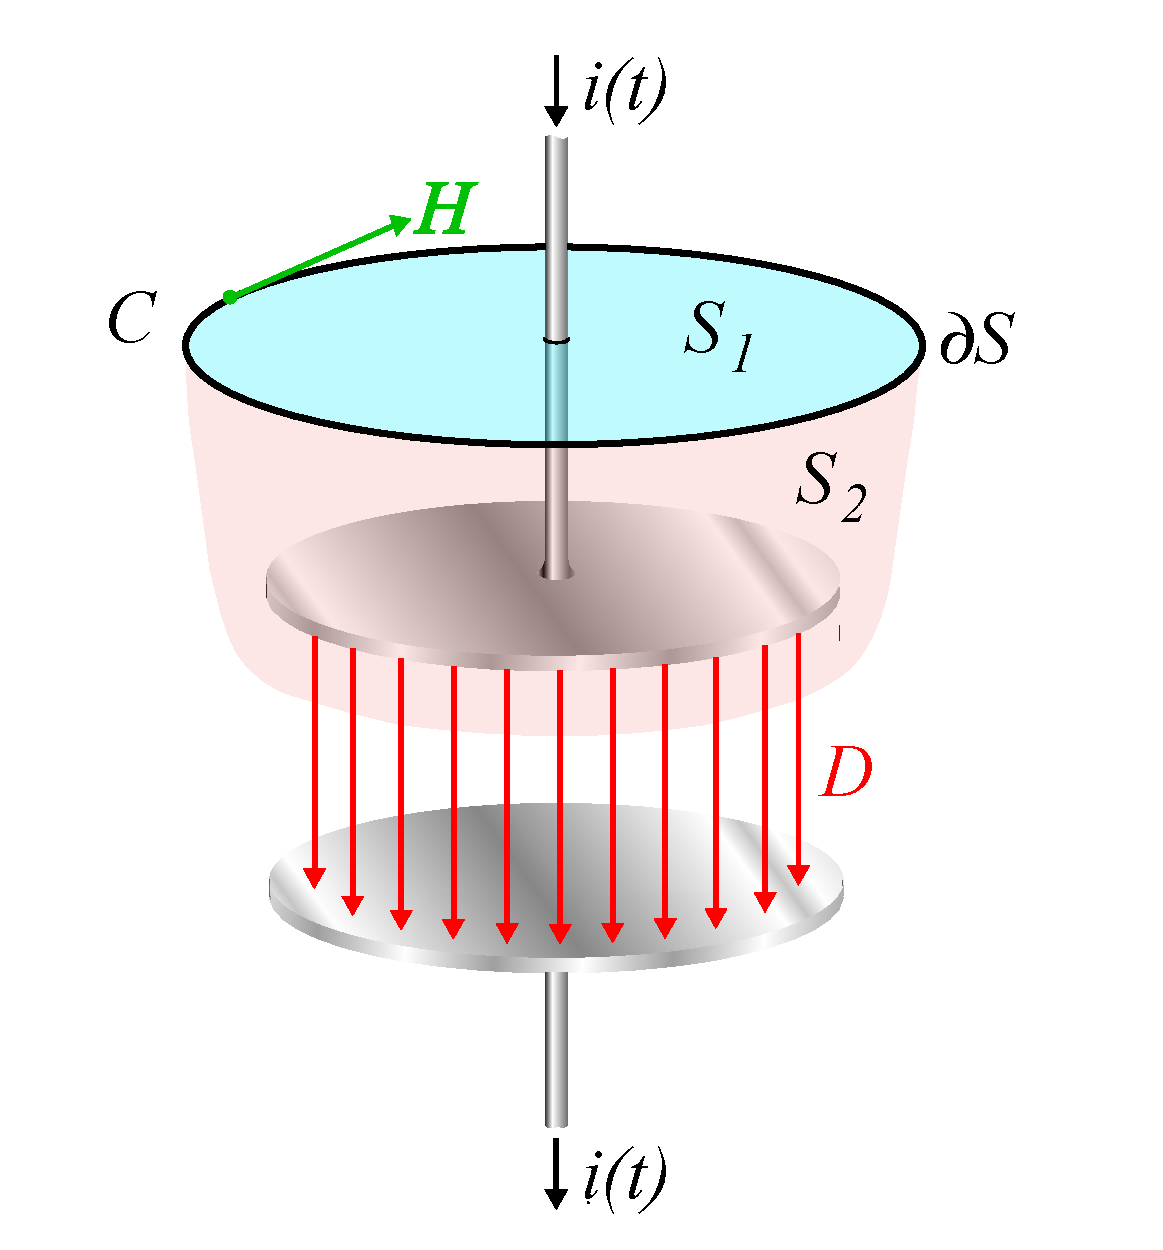
\includegraphics[width=7cm]{image/Displacement_current_in_capacitor.pdf}
\end{Figure}
在$S_1$上适用安培环路定律,由于通过$S_1$的电流是$i(t)$
\begin{Equation}&[3]
    \Ilot[C]\vb*{H}\cdot\dd{\vb*{l}}=i(t)
\end{Equation}
在$S_2$上适用安培环路定律,由于通过$S_2$的电流是$0$
\begin{Equation}
    \Ilot[C]\vb*{H}\cdot\dd{\vb*{l}}=0
\end{Equation}
但是,磁场强度$\vb*{H}$在同一闭合曲线$C$上的环流不可能同时为$i(t)$和$0$,产生矛盾。针对该问题,麦克斯韦认为,电容器的两个极板间必然存在另一种形式的电流。电容器极板间电荷分布随着时间变化,电容极板间形成时变电场,麦克斯韦位移电流假设就在于,他认为,\empx{时变电场也是电流},称为\uwave{位移电流}(Displacement Current),区别于\uwave{传导电流}(Conduction Current)。

将\fancyref{ppt:电介质中的高斯定律}代入\fancyref{eqt:电流连续性方程}
\begin{Equation}&[4]
    \div\vb*{J}=-\pdv{\rho}{t}=-\pdv{t}\qty(\div\vb*{D})=-\div\pdv{\vb*{D}}{t}
\end{Equation}
即
\begin{Equation}&[5]
    \div(\vb*{J}+\pdv{\vb*{D}}{t})=0
\end{Equation}
这里$\pdv*{\vb*{D}}{t}$是电位移随时间的变化率,称为位移电流密度,记作$\vb*{J}_\text{d}$。

这里\xrefpeq{5}重新诠释了电流连续性方程,在过去的版本中,电流场只有在恒定条件下才是连续的,电流在电荷密度发生变化处产生源和汇,在新的观点下,我们认为电流应当要同时包含传导电流和位移电流,这样即便在时变电磁场的情形下,电流也都是连续的了。如果回到前面电容的例子,在导线上电流以运动电荷的传导电流的形态进行传输,在电容中电流以时变电场的位移电流的形态进行传输,两者大小相等,形成连续的电流,尽管电容中没有任何导线。

而位移电流和传导电流一样,均需要产生磁场,因而安培环路定律需要修正为
\begin{Equation}&[6]
    \curl\vb*{H}=\vb*{J}+\pdv{\vb*{D}}{t}
\end{Equation}
现在两端取散度就不会再出现任何矛盾了,考虑到\xrefpeq{5}的结果。

而如果我们抛开位移电流这些表象,其实\xrefpeq{6}就告诉我们,时变电场产生磁场。
\begin{BoxProperty}[时变电场产生涡旋磁场]
    时变电场,是磁场的正涡旋源
    \begin{Equation}
        \grad\times\vb*{H}=\vb*{J}+\pdv{\vb*{D}}{t}
    \end{Equation}
\end{BoxProperty}

这里我们或许会想,为什么“变化的电场”的效果可以等效为位移电流,而“变化的磁场”的效果则不能等效为某种古怪的电荷?这种不对称性来自哪里?关键是在于,变化的电场和磁场总是充当对方的涡旋源,但在静电学和静磁学理论中,电场的源是电荷,磁场的源是电流
\begin{itemize}
    \item 电流是磁场的涡旋源,因此变化电场产生的磁场的涡旋源可以视作某种电流。
    \item 电荷是电场的通量源,因此变化磁场产生的电场的涡旋源不能视作某种电荷。
\end{itemize}